\section{Parametrisation of PDEs}

Parametrised PDEs find applications across numerous scientific and engineering domains, including fluid dynamics, structural mechanics, electromagnetics, and more. They provide a powerful framework for modelling complex phenomena where multiple factors influence the system's behaviour. Parameterised PDEs introduce additional parameters $\bm{\mu}$ into the equation, allowing for a more flexible representation of physical systems. These parameters can represent various factors such as material properties, boundary conditions, or geometric features. By incorporating parameters, the PDEs become functions of these variables, enabling the analysis of how changes in parameters affect the system's behaviour. 

The materials parameters $\bm{\mu}_m$ intuitively refer to the varying material properties in the problem. The boundary conditions parameters $\bm{\mu}_b$ refer to variables that influence the boundary conditions imposed on the problem. The geometric parameter $\bm{\mu}_g$ refers to a variable that represents the geometric features or configurations of the system being modelled. These parameters capture aspects such as the shape, size, orientation, or position of geometric entities within the domain of the PDE.

For demonstration purposes, this project focuses on working on a fixed geometric domain of a 1 by 1 grid. The mixed formulation problem is defined with the following conditions: 

\begin{align}
    u = 0 \quad & {\rm on} \ \Gamma_{D} = \{(0, y) \cup (1, y) \in \partial \Omega\} \label{eqn:set_bc} \\
    \text{Flux: }  g = & \sin(\mu_1 x)  \quad {\rm on} \ \Gamma_{N} = \{(x, 0) \cup (x, 1) \in \partial \Omega\} \label{eqn:set_flux} \\   
    \text{Source: } f & = \mu_2 \, \exp \{-\mu_3[(x-\mu_4)^2 + (y-\mu_5)^2]\}  \label{eqn:source}
\end{align}

In this particular case, Equations \ref{eqn:set_bc} and \ref{eqn:set_flux} specify the boundary conditions. The flux exhibits a sinusoidal wave pattern at the top and bottom, while the function $u$ is constrained to zero at the left and right boundaries.
Equation \ref{eqn:source} defines the behaviour of the source, where $u$ exhibits an exponential decay depending on how far away it is from the source.

Solutions are then compared with different initialisations of $\mu_i$. During the early stages of the project, we focused on changing all five parameters $\mu_i, \text{where } i \in \{1, 2, 3, 4, 5\}$.  As a based case for comparison, the parameters are set to be $\bm{\mu} = [5, 10.0, 50.0, 0.5, 0.5]$. Figure \ref{fig: base} shows the behaviours of the scalar and the flux term under the base case. The parameters were then varied and the effect of each $\mu_i$ are found below, based on results from Figure \ref{fig:all_solutions}:

\begin{itemize}
    \item $\mu_1$ controls the frequency of the flux boundary. Larger $\mu_1$ leads to a higher changing flux at the boundary, and more changes are imposed on $u$ around the flux boundary.  
    \item $\mu_2$ scales the overall amplitude of $u$. The flux would also increase with a  larger $\mu_2$, especially in between the source and the boundary, where $u = 0$ is fixed. 
    \item $\mu_3$ controls the decay rate of the propagation of $u$ from the source. For smaller $\mu_3$, $u$ is larger in unconstrained regions. However, due to fixed boundary conditions, the flux is larger at some regions near the boundary, counterfeiting the effect of smaller decay.  
    \item $\mu_4$ and $\mu_5$ simply control the source position. 

\end{itemize}

\begin{figure}[!h]
        \begin{center}
	\begin{subfigure}{0.4\linewidth}
		\centering
		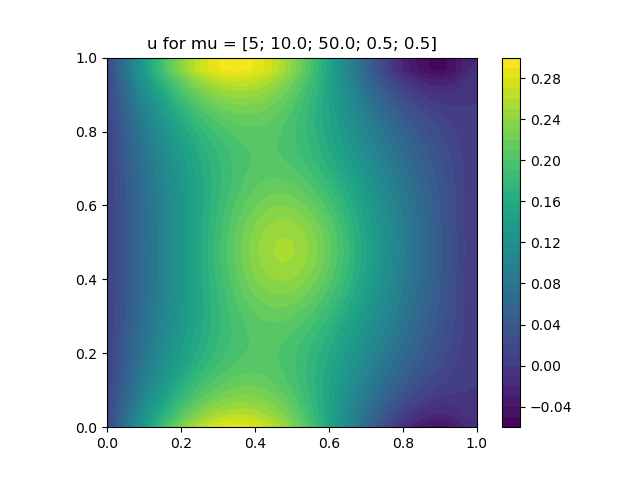
\includegraphics[width=\linewidth]{figs/mixed_u_mu1.png}
            \caption{base case u}
		\label{fig: base_u}
	\end{subfigure}
	\begin{subfigure}{0.4\linewidth}
		\centering
		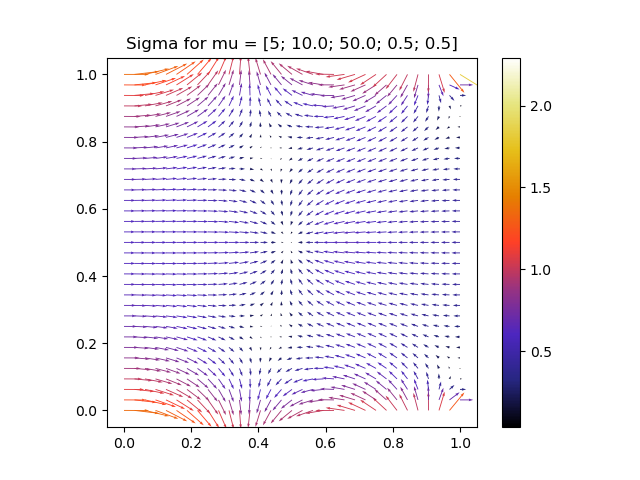
\includegraphics[width=\linewidth]{figs/mixed_sigma_mu1.png}
            \caption{base case $\sigma$}
		\label{fig: base_sig}
	\end{subfigure}
	\caption{Base case solutions for $\bm{\mu} = [5; 10.0; 50.0; 0.5; 0.5]$}
	\label{fig: base}
        \end{center}
\end{figure}

\begin{figure}[!htb]
    \centering
    \begin{subfigure}{0.35\linewidth}
        \centering
        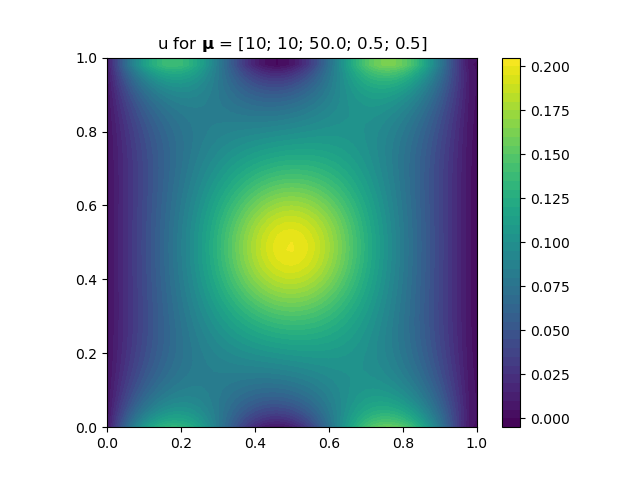
\includegraphics[width=\linewidth]{figs/mixed_u_mu11.png}
        \subcaption{Solution for u,  $\mu_1 = 10$}
        \label{subfig:mu11_a}
    \end{subfigure}%
    \begin{subfigure}{0.35\linewidth}
        \centering
        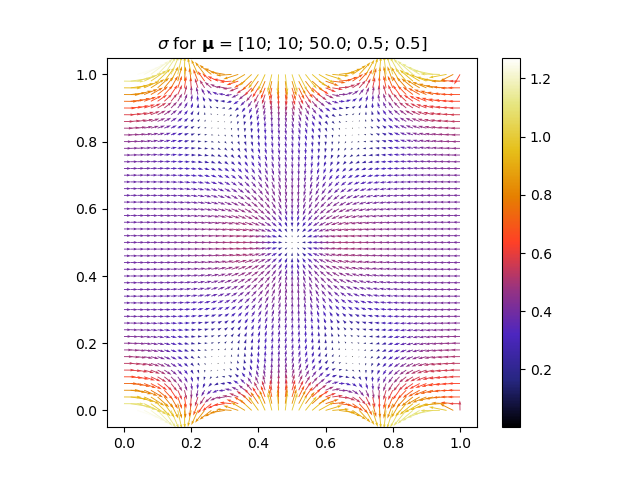
\includegraphics[width=\linewidth]{figs/mixed_sig_mu11.png}
        \subcaption{Solution for $\sigma$ , $\mu_1 = 10$}
        \label{subfig:mu11_b}
    \end{subfigure}%
    \begin{subfigure}{0.35\linewidth}
        \centering
        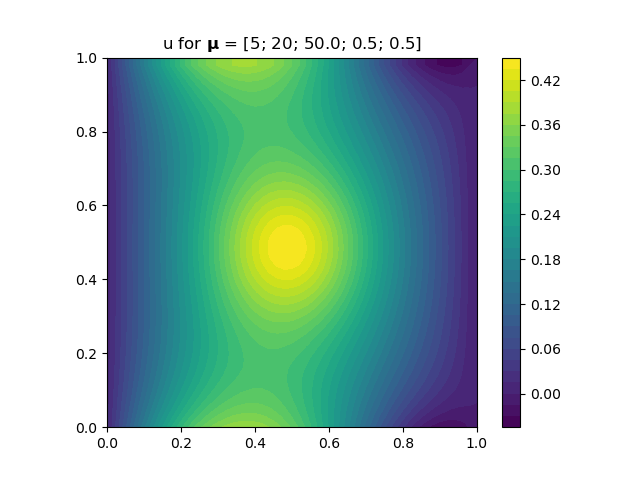
\includegraphics[width=\linewidth]{figs/mixed_u2_mu2.png}
        \subcaption{Solution for u, $\mu_2 = 20$}
        \label{subfig:mu2_a}
    \end{subfigure}
    \begin{subfigure}{0.35\linewidth}
        \centering
        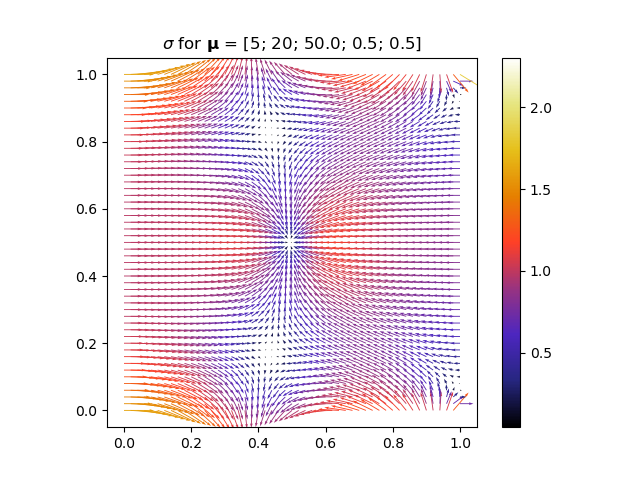
\includegraphics[width=\linewidth]{figs/mixed_sigma2_mu2.png}
        \subcaption{Solution for $\sigma$, $\mu_2 = 20$}
        \label{subfig:mu2_b}
    \end{subfigure}%
    \begin{subfigure}{0.35\linewidth}
        \centering
        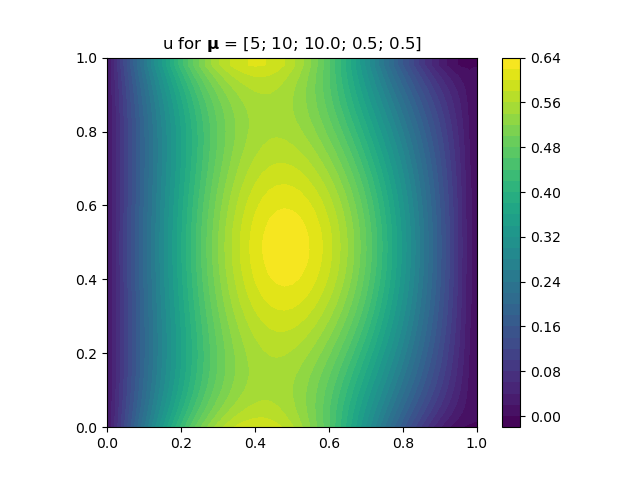
\includegraphics[width=\linewidth]{figs/mixed_u_mu3.png}
        \subcaption{Solution for u, $\mu_3 = 10$}
        \label{subfig:mu3_a}
    \end{subfigure}%
    \begin{subfigure}{0.35\linewidth}
        \centering
        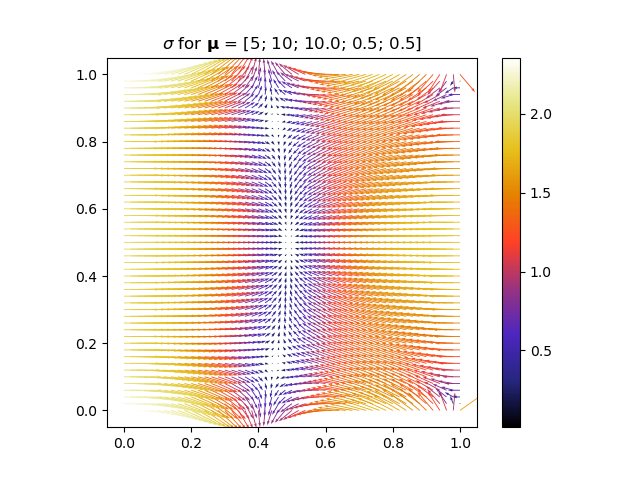
\includegraphics[width=\linewidth]{figs/mixed_sig_mu3.png}
        \subcaption{Solution for $\sigma$ , $\mu_3 = 10$}
        \label{subfig:mu3_b}
    \end{subfigure}
    \begin{subfigure}{0.4\linewidth}
        \centering
        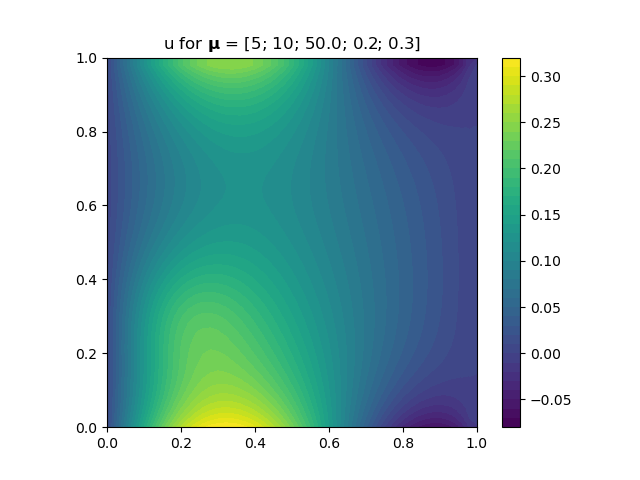
\includegraphics[width=\linewidth]{figs/mixed_u_mu45.png}
        \subcaption{Solution for u, $\mu_4, \mu_5 = 0.2, 0.3$}
        \label{subfig:mu45_a}
    \end{subfigure}
    \begin{subfigure}{0.4\linewidth}
        \centering
        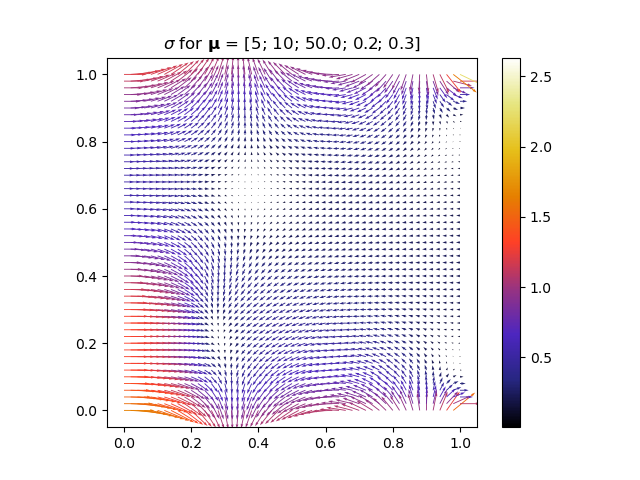
\includegraphics[width=\linewidth]{figs/mixed_sig_mu45.png}
        \subcaption{Solution for $\sigma$ , $\mu_4, \mu_5 = 0.2, 0.3$}
        \label{subfig:mu45_b}
    \end{subfigure}
    
    \caption{Solutions for different parameter variations with base case $\bm{\mu} = [5; 10.0; 50.0; 0.5; 0.5]$}
    \label{fig:all_solutions}
\end{figure}

As the project progressed, we observed that certain parameters had a greater influence on the variability of the solution manifolds. Notably, through extensive experimentation, it was observed that the parameters $\mu_3$, $\mu_4$, and $\mu_5$ exhibited considerable fluctuations in the solution. These fluctuations led to a major issue during the later stage of the project, where the MOR procedure could not accurately capture the dominant modes of the solutions, particularly in reducing the dimensionality of the solution for $\sigma$

Consequently, to streamline the analysis, we decided to simplify the problem formulation. In this revised approach, the investigation would primarily concentrate on the parameters $\mu_1$ and $\mu_2$, as they were found to have a more pronounced impact on the solution behaviour and a better level of controllability. By narrowing the focus to these key parameters, the complexity of the problem could be effectively reduced while still capturing the essential dynamics and trends. This allows us to study the effectiveness of the POD-ANN approach more closely. 

The effect of the number of parameters on the accuracy of POD will be discussed in more detail in the next session, where we will provide concrete numerical results to support our stand of using only two parameters.



\newpage